\documentclass[11pt]{article}
\usepackage{amsmath, amssymb, amsthm}
\usepackage{geometry}
\usepackage{hyperref}
\usepackage{tikz}
\usetikzlibrary{arrows.meta, positioning, shapes.geometric}
\geometry{margin=1in}

\title{Notes 00 \\ Review of Statistics: \\ Multivariate Analysis (PCA, Factor Analysis, Canonical Correlation)}
\author{DATA 000: Advanced Computational Methods in Education and the Social Sciences}
\date{Alexander \\ Spring 2026}

\begin{document}

\maketitle

\tableofcontents

\section{Introduction}

\textbf{Multivariate analysis} refers to statistical techniques that analyze more than two variables simultaneously to uncover relationships, patterns, or structure in the data\ [1][2][3][5][6]. These methods are essential in education and the social sciences, where phenomena are often influenced by many factors at once.

\section{Overview: Types of Multivariate Analysis}

\begin{itemize}
    \item \textbf{Dependence techniques:} Explore relationships where some variables are dependent on others (e.g., multiple regression, MANOVA).
    \item \textbf{Interdependence techniques:} Explore relationships without designating dependent/independent variables, seeking patterns or groupings (e.g., PCA, factor analysis, cluster analysis)\ [1][2][5][7].
\end{itemize}

\section{Principal Component Analysis (PCA)}

\subsection{Purpose}

PCA is a technique for reducing the dimensionality of a dataset by transforming original variables into a new set of uncorrelated variables (principal components) that capture the maximum variance\ [1][2][5].

\subsection{How PCA Works}

\begin{enumerate}
    \item Standardize the variables (if measured on different scales).
    \item Compute the covariance or correlation matrix.
    \item Find the eigenvalues and eigenvectors.
    \item Principal components are ordered by the amount of variance they explain.
\end{enumerate}

\subsection{Mathematical Formulation}

Given data matrix $\mathbf{X}$ (centered):

\[
\mathbf{Z} = \mathbf{X} \mathbf{W}
\]
where:
\begin{itemize}
    \item $\mathbf{W}$ = matrix of eigenvectors (principal axes)
    \item $\mathbf{Z}$ = principal component scores
\end{itemize}

\subsection*{Visualization: PCA Axes}
\begin{center}
\begin{tikzpicture}[scale=1.2]
  % Axes
  \draw[->] (-2,0) -- (2,0) node[right] {$X_1$};
  \draw[->] (0,-2) -- (0,2) node[above] {$X_2$};
  % Data cloud
  \foreach \x/\y in {-1.4/-1.2, -1.1/-0.8, -0.8/-0.7, -0.5/-0.2, 0.1/0.2, 0.5/0.6, 0.9/1.2, 1.3/1.5} {
    \filldraw[blue] (\x,\y) circle (1.5pt);
  }
  % PC1
  \draw[thick, red, ->] (0,0) -- (1.3,1.3) node[above right] {PC1};
  % PC2
  \draw[thick, green!70!black, ->] (0,0) -- (-1.3,1.3) node[above left] {PC2};
\end{tikzpicture}
\end{center}

\subsection{Example: Education (with Solution)}

\textbf{Scenario:} A researcher collects math, reading, and science test scores for 100 students. PCA is used to reduce these to a single index of "academic achievement."

\textbf{Solution:}
- Standardize scores.
- Compute covariance/correlation matrix.
- Extract first principal component (PC1), which might load equally on all three subjects if they are highly correlated.
- PC1 scores can be used as a composite achievement score for further analysis.

\subsection{Interpretation}

- The first principal component explains the largest possible variance.
- Subsequent components explain remaining variance, are uncorrelated with previous ones.

\section{Factor Analysis}

\subsection{Purpose}

Factor analysis seeks to identify underlying latent variables (factors) that explain the pattern of correlations among observed variables\ [1][2][5][6].

\subsection{Model}

\[
X_j = \lambda_{j1}F_1 + \lambda_{j2}F_2 + \cdots + \lambda_{jm}F_m + \epsilon_j
\]
where:
\begin{itemize}
    \item $X_j$ = observed variable
    \item $F_m$ = latent factors
    \item $\lambda_{jm}$ = factor loadings
    \item $\epsilon_j$ = unique variance (error)
\end{itemize}

\subsection*{Visualization: Factor Model}
\begin{center}
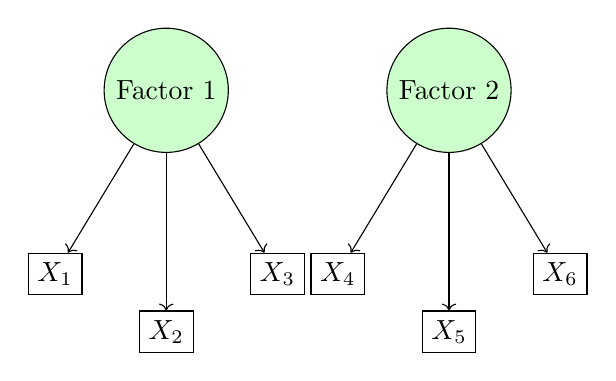
\begin{tikzpicture}[scale=1, node distance=2cm]
  \node (F1) [circle, draw, fill=green!20] {Factor 1};
  \node (F2) [circle, draw, fill=green!20, right=of F1] {Factor 2};
  \node (X1) [rectangle, draw, below left=1.5cm and 0.5cm of F1] {$X_1$};
  \node (X2) [rectangle, draw, below=of F1] {$X_2$};
  \node (X3) [rectangle, draw, below right=1.5cm and 0.5cm of F1] {$X_3$};
  \node (X4) [rectangle, draw, below left=1.5cm and 0.5cm of F2] {$X_4$};
  \node (X5) [rectangle, draw, below=of F2] {$X_5$};
  \node (X6) [rectangle, draw, below right=1.5cm and 0.5cm of F2] {$X_6$};
  \draw[->] (F1) -- (X1);
  \draw[->] (F1) -- (X2);
  \draw[->] (F1) -- (X3);
  \draw[->] (F2) -- (X4);
  \draw[->] (F2) -- (X5);
  \draw[->] (F2) -- (X6);
\end{tikzpicture}
\end{center}

\subsection{Example: Social Science (with Solution)}

\textbf{Scenario:} A survey measures six items related to "job satisfaction." Factor analysis is used to see if these items group into underlying dimensions.

\textbf{Solution:}
- Correlation matrix shows two clusters of items.
- Factor analysis extracts two factors: "Work Environment" and "Compensation."
- Factor loadings indicate which items load on which factor.
- Researchers can use factor scores for further analysis or reporting.

\subsection{Interpretation}

- Factors are latent constructs that summarize patterns in observed variables.
- Factor loadings show the strength of association between each variable and factor.

\section{Canonical Correlation Analysis (CCA)}

\subsection{Purpose}

CCA explores the relationship between two sets of variables, finding linear combinations (canonical variates) that are maximally correlated\ [1][2][5][6][8].

\subsection{Model}

Given two sets of variables, $\mathbf{X}$ and $\mathbf{Y}$:

\[
U = a_1 X_1 + a_2 X_2 + \cdots + a_p X_p
\]
\[
V = b_1 Y_1 + b_2 Y_2 + \cdots + b_q Y_q
\]
CCA finds coefficients $a_i$ and $b_j$ so that the correlation between $U$ and $V$ is maximized.

\subsection*{Visualization: Canonical Correlation}
\begin{center}
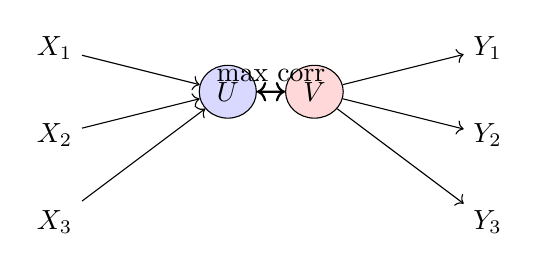
\begin{tikzpicture}[scale=1.1]
  % X set
  \node (X1) at (0,2) {$X_1$};
  \node (X2) at (0,1) {$X_2$};
  \node (X3) at (0,0) {$X_3$};
  % Y set
  \node (Y1) at (5,2) {$Y_1$};
  \node (Y2) at (5,1) {$Y_2$};
  \node (Y3) at (5,0) {$Y_3$};
  % Canonical variates
  \node[ellipse, draw, fill=blue!15] (U) at (2,1.5) {$U$};
  \node[ellipse, draw, fill=red!15] (V) at (3,1.5) {$V$};
  % Arrows
  \foreach \from in {X1,X2,X3}
    \draw[->] (\from) -- (U);
  \foreach \to in {Y1,Y2,Y3}
    \draw[->] (V) -- (\to);
  \draw[<->, thick] (U) -- (V) node[midway, above] {max corr};
\end{tikzpicture}
\end{center}

\subsection{Example: Education (with Solution)}

\textbf{Scenario:} A researcher wants to relate a set of academic measures (math, reading, science scores) to a set of psychosocial measures (motivation, self-esteem, attendance).

\textbf{Solution:}
- CCA finds linear combinations of academic and psychosocial variables that are most strongly correlated.
- The first canonical correlation might show that high academic achievement is associated with high motivation and attendance.
- Interpretation helps understand the multivariate relationship between two domains.

\section{Summary Table: Multivariate Methods}

\begin{tabular}{|l|l|l|l|}
\hline
\textbf{Method} & \textbf{Purpose} & \textbf{Variables} & \textbf{Example Use} \\
\hline
PCA & Reduce dimensionality & Many observed & Composite achievement score \\
Factor Analysis & Uncover latent structure & Many observed & Job satisfaction factors \\
Canonical Correlation & Relate two sets & Two sets & Academic $\leftrightarrow$ psychosocial \\
\hline
\end{tabular}

\section{Further Notes}

\begin{itemize}
    \item Multivariate analysis is essential for understanding complex, real-world data\ [1][2][3][5][6].
    \item Always check assumptions (e.g., linearity, normality, sample size).
    \item Interpretation should be guided by theory and context.
    \item Software (R, Python, SPSS) is typically used for computation.
\end{itemize}

\end{document}
